\documentclass[tikz,border=2pt]{standalone}
\usepackage{amsmath,amssymb}
\usepackage{tikz}
\usetikzlibrary{arrows.meta}

\begin{document}
% The prosecutor's fallacy confuses P(match | innocent) with P(innocent | match). With a
% match probability of 1 in 100 000 in a city of 1 000 000, about 10 innocent people match
% besides the one culprit, so a match alone leaves P(innocent | match) near 10/11.
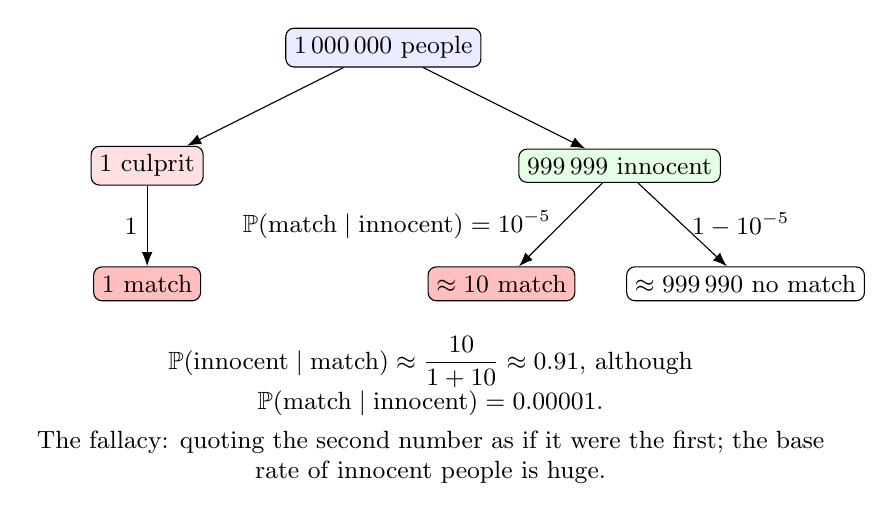
\begin{tikzpicture}[every node/.style={font=\small}, >={Latex[length=1.8mm]}, lvl/.style={draw, rounded corners=3pt, inner sep=3pt}]
	\node[lvl, fill=blue!8] (root) at (0,0) {$1\,000\,000$ people};
	\node[lvl, fill=red!12] (G) at (-3,-1.5) {$1$ culprit};
	\node[lvl, fill=green!10] (I) at (3,-1.5) {$999\,999$ innocent};
	\draw[->] (root) -- (G);
	\draw[->] (root) -- (I);
	\node[lvl, fill=red!25] (GM) at (-3,-3) {$1$ match};
	\node[lvl, fill=red!25] (IM) at (1.5,-3) {$\approx10$ match};
	\node[lvl] (IN) at (4.6,-3) {$\approx999\,990$ no match};
	\draw[->] (G) -- (GM) node[midway, left] {$1$};
	\draw[->] (I) -- (IM) node[midway, left] {$\mathbb{P}(\text{match}\mid\text{innocent})=10^{-5}$};
	\draw[->] (I) -- (IN) node[midway, right] {$1-10^{-5}$};
	\node[anchor=north, align=flush center, text width=10cm] at (0.6,-3.55) {$\mathbb{P}(\text{innocent}\mid\text{match})\approx\dfrac{10}{1+10}\approx0.91$, although $\mathbb{P}(\text{match}\mid\text{innocent})=0.00001$.\\[3pt] The fallacy: quoting the second number as if it were the first; the base rate of innocent people is huge.};
\end{tikzpicture}
\end{document}
